\section{Motivation}

Breast cancer is one of the most common forms of cancer amongst women in the UK, with statistics indicating that 1 in 7 females will be diagnosed with breast cancer in their lifetime. Indeed, 55,200 new breast cancer cases are reported every year in the UK, of which a disheartening average of 11,400 lead to death \citep{BreastCancerResearchUK}. With an average of 20\% mortality rate, breast cancer is ranked as one of the deadliest diseases.\\

Early detection of breast cancer through screening tests such as mammograms is an efficient way to maximise patients' survival rate by treating the disease prematurely. However, no matter the expertise of radiologists examining mammograms, external factors such as fatigue, distractions and human error need to be minimised \citep{Polat2007}, as the rate of missed breast cancers during initial mammogram screenings  are as high as 30\% \citep{Elter2009}. To convey the complexity of mammogram interpretation, Figure~\ref{fig:introduction-mammogram-examples} illustrates three different mammograms containing either normal or abnormal (benign and malignant) cases, and how similar they all look to an untrained eye.\\

\begin{figure}[ht]
\centerline{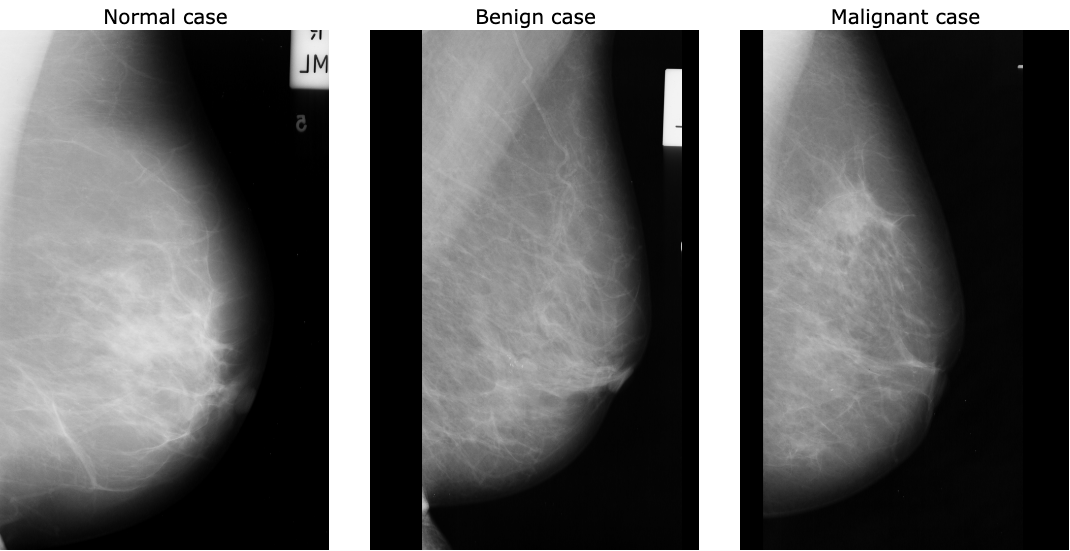
\includegraphics[width=\textwidth]{figures/introduction/mammogram examples.png}}
\caption{\label{fig:introduction-mammogram-examples}Example of three types of mammograms, including normal, benign and malignant cases. Figures extracted from the mini-MIAS dataset (Suckling, 1994). Created using draw.io.}
\end{figure}

Error-prone mammogram interpretations by radiologists can lead to decisions that can ultimately harm the patients. If a mammogram is diagnosed as malignant, breast biopsies (extraction of cells in breast tissue) are usually prescribed. However, 40-60\% of biopsies are diagnosed as benign, clearly betraying the necessity for correct mammography diagnosis to avoid needless operations, anxiety and pain for the patients \citep{Hepsag2017}. On the one hand, breast cancers can be missed altogether, inducing an absence of treatments for sick patients, while on the other hand, an instance of breast cancer can be reported when in reality there is no cancerous tumour, leading to unnecessary treatment being carried out \citep{Elter2009}.\\

To that end, using Computer-Assisted Detection (CAD) software can help minimise the number of wrong interpretations and increase the accuracy of mammography screening \citep{Shen2017}.\\

The motivation behind this project is to explore techniques for implementing a deep learning system that can accurately detect breast cancer in order to prevent late treatments due to false negatives as well as preventing unnecessary treatments in cases of false positives. Ultimately, the long-term target of this project is to combine it with other deep learning algorithms developed across other projects supervised by Dr David Harris-Birtill (past and present). This will allow a general artificial intelligence system capable of detecting multiple forms of cancer with higher accuracies than radiologist diagnoses.\\

%%%%%%%%%%%%%%%%%%%%%%%%%%%%%%%%%%%%%%%%%%%%%%%%%%%%%%%%%%%%%%%%%%%%%%%%%%%%%%%%%%

\section{Problem Description}
\label{sec:problem-description}

CAD systems using deep learning techniques could, in theory, highly increase the accuracy of mammogram screenings for detecting early signs of breast cancers. However, these techniques require large amounts of data to learn the cancer's underlying patterns and adapt to new cases, and require  powerful computing resources to accelerate the process of learning the data, making them very hard to optimise.\\

Parts of the work undertaken during this project will be conducted as a group comprised of two other members, Ashay Patel and Shuen-Jen Chen. Section~\ref{sec:introduction-objectives} covers which tasks will be conducted personally/in a group in more detail. The reasoning behind these common tasks is for a functional pipeline to be reached earlier, eventually allowing each group member to further explore deep learning techniques individually more quickly due to the limited time frame of this project, using the common primary pipeline as a baseline.

%%%%%%%%%%%%%%%%%%%%%%%%%%%%%%%%%%%%%%%%%%%%%%%%%%%%%%%%%%%%%%%%%%%%%%%%%%%%%%%%%%

\section{Objectives}
\label{sec:introduction-objectives}

The main objective of this project consists of implementing a deep learning pipeline that will be able to learn how to detect cases of breast cancer in mammograms. This objective is broken down into two steps:
\begin{itemize}
    \item \textbf{Group work}: a common deep learning pipeline will be initially implemented as part of a group with Ashay Patel and Shuen-Jen Chen over the course of a three-week period, including data cleaning and pre-processing, results output and a basic deep learning model. The distribution of tasks between the group can be found in Appendix~\ref{ch:appendix-team-meeting-summaries}.
    \item \textbf{Individual work}: the pipeline above will then be individually extended and evaluated by using various deep learning techniques.
\end{itemize}

An extensive context survey has to first be conducted to cover the background of deep learning techniques applied to the field of cancer detection and to review existing results. This includes identifying results achieved using different methods (e.g. traditional machine learning techniques). This step is primordial as it will guide the research towards the most promising areas, as well as govern the choice of techniques to implement and explore in further chapters.\\

Finally, the final results achieved individually will be compared with the baseline pipeline created as a group, as well as the results found in papers that used the same datasets.

%%%%%%%%%%%%%%%%%%%%%%%%%%%%%%%%%%%%%%%%%%%%%%%%%%%%%%%%%%%%%%%%%%%%%%%%%%%%%%%%%%

\section{Report Structure}

\tab \textbf{Introduction} \space 
Presents an overview of the subject's background through the problem description and the motivation behind this project, followed by the objectives that the project aims to achieve.\\

\textbf{Context Survey} \space
Explores the literature and background surrounding breast cancer detection techniques, starting from primitive cancer detection systems, followed by traditional machine learning methods, and ending with the deep learning techniques that have been recently used.\\

\textbf{Ethics \& Datasets} \space
Considers the ethical issues taken into account for this project and describes the datasets used.\\

\textbf{Design} \space
Explores high-level design considerations regarding the deep learning pipeline to implement and the software in general.\\

\textbf{Implementation} \space
Comprehensively covers the steps followed when implementing the deep learning pipeline, explaining the practical solutions followed.\\

\textbf{Evaluation} \space
Reviews the different results to assess the efficiency of the different techniques used to train the model and how it compares to other models, including the common pipeline, the baseline and relevant results identified in the context survey.\\

\textbf{Conclusions} \space
Summarises the project's accomplished objectives, its limitations, plans for future work, and a final reflection on the project as a whole.
